\documentclass[dvipdfmx]{jsarticle}

\usepackage{silence}
\WarningFilter{caption}{Unknown document}

\usepackage{amsmath}
\usepackage{amssymb}
\usepackage{amsthm}
\usepackage{ascmac}
\usepackage{bm}
\usepackage{float}
\usepackage{graphicx}
\usepackage{hyperref}
\usepackage{latexsym}
\usepackage{listings}
\usepackage{mathtools}
\usepackage{multicol}
\usepackage{subcaption}
\usepackage{tcolorbox}
\usepackage{xcolor}

\makeatletter
% 図番号を"<章番号>.<図番号>" へ
\renewcommand{\thefigure}{\thesubsection.\arabic{figure}}
\renewcommand{\thetable}{\thesubsection.\arabic{table}}
% 章が進むごとに図番号をリセットする
\@addtoreset{figure}{section}
\@addtoreset{table}{section}
\@addtoreset{figure}{subsection}
\@addtoreset{table}{subsection}
\makeatother
% TODO
\newcommand{\todo}[1]{\textcolor{magenta}{TODO: #1}}
% ソースコードの表示設定
\lstset{
    language={bash},
    basicstyle={\ttfamily\small},
    keywordstyle={\color{blue}},
    commentstyle={\color{green}},
    stringstyle=\color{red},
    tabsize=4,
    breaklines=true,
}

% Title
\title{Chibicraft}
\author{
    慶應義塾大学 環境情報学部 \\
    72375699 二又康輔
}
\date{\today}

% Document
\begin{document}
\maketitle

% Contents
\section{概要}
Chibicraftは「できるだけフルスクラッチでMinecraftを再現する」ことを目標として作られたゲームである。
現在の機能としては、主にワールドの探索、ブロックの配置、破壊を行うことができる。

\begin{figure}[H]
    \begin{center}
        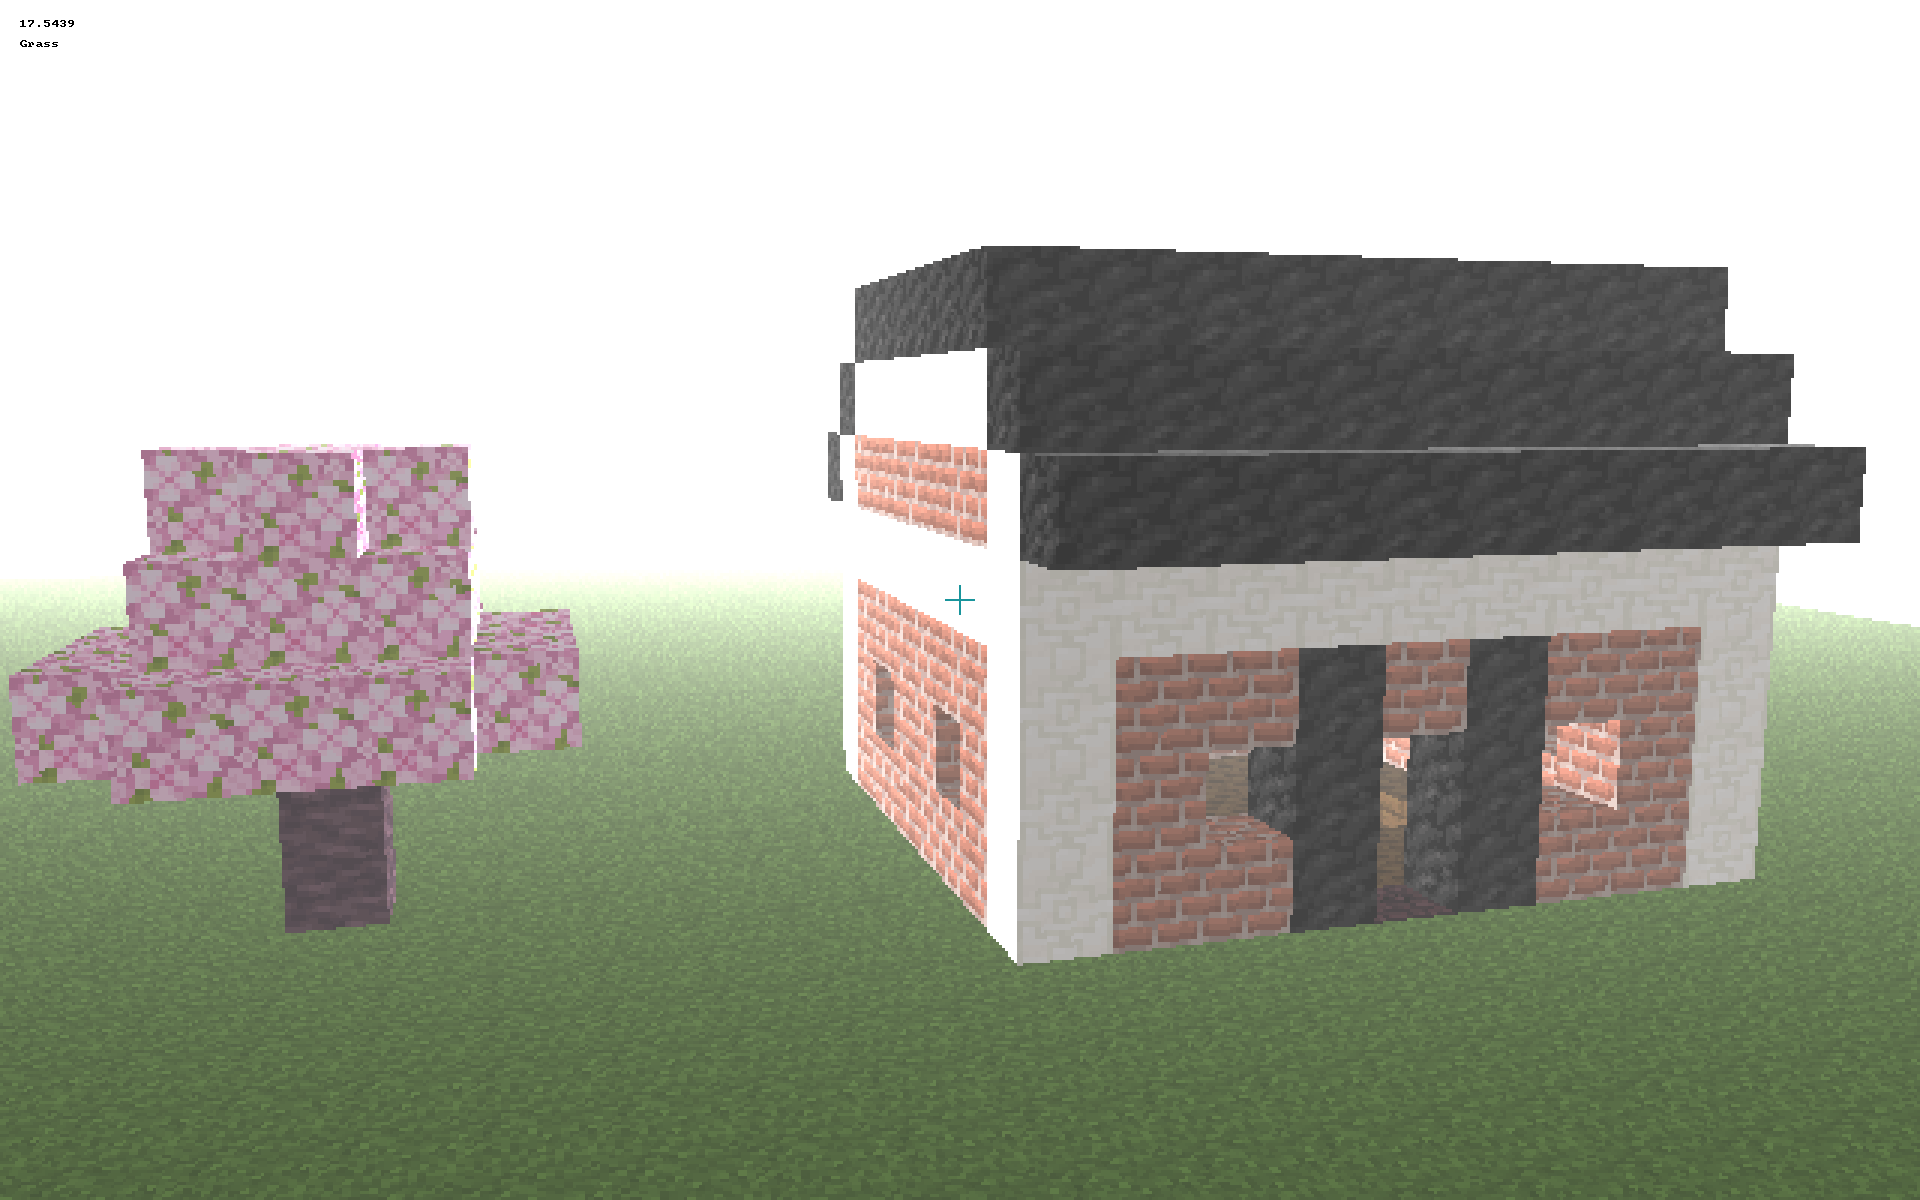
\includegraphics[width=100mm]{chibi.png}
        \caption{Chibicraftのイメージ}
    \end{center}
\end{figure}

\section{環境構築}
Chibicraftは現在、Ubuntu22.04上で正常に動作することが確認されている。
また、Kali Linux2024.1上では、動作はするが視点操作が反転するというバグが発見されている。
Mac OSやWindows上での動作は保証されていないため、Virtual Machine等を用いてUbuntu上で動かすことを推奨している。

\subsection{Ubuntu上での環境構築手順}
まず、SDL1.2とOpenGL Mathematicsをインストールする。
\begin{lstlisting}
$ sudo apt update
$ sudo apt install libsdl1.2-dev -y
$ sudo apt install libglm-dev -y
\end{lstlisting}
次にChibicraftをインストールする。
\begin{lstlisting}
$ git clone --recursive https://github.com/matajupi/chibigit.git
$ cd Chibicraft
$ make
\end{lstlisting}
ChibicraftはChibicraftディレクトリ直下で次のコマンドを実行することにより起動することができる。
\begin{lstlisting}
$ ./bin/chibi
\end{lstlisting}

\section{ゲームの操作}
\begin{tabular}{ll}                                         \hline
    キー            & 説明                                  \\ \hline \hline
    w               & 前進                                  \\
    s               & 後退                                  \\
    a               & 左に移動                              \\
    d               & 右に移動                              \\
    マウスカーソル  & 視点操作                              \\
    左クリック      & ブロックを破壊                        \\
    右クリック      & ブロックを配置                        \\
    左矢印          & ブロックの変更(種類は画面左上に表示)  \\
    右矢印          & ブロックの変更(種類は画面左上に表示)  \\ \hline
\end{tabular}

\section{アピールしたい点}
ChibicraftはC++で書かれており、ゲームエンジンにQuickCG\cite{quickcg}を利用している。
ChibicraftはできるだけフルスクラッチでMinecraftを再現することを目標としているため、3D描画に特化したゲームエンジンやライブラリ等は利用していない。
また、LLMも利用していない。
3Dの描画にはRaycastingというシンプルなアルゴリズムを用いている。
また、Raycastingの高速化のためにOpenMPによる並列化を行っている。

\begin{thebibliography}{1}
    \bibitem{quickcg} QuickCG
    \url{https://lodev.org/quickcg/}
\end{thebibliography}

\end{document}
